% =====================================================================
\chapter{Arbitrage de base, \emph{cash-and-carry} et \emph{funding}}
\label{ch:14}
% =====================================================================

\section{Objectifs et organisation du chapitre}

\paragraph{Objectifs.} Le chapitre~13 a montré que l'arbitrage pur entre plateformes est une course perdue d'avance pour un particulier. Les quasi-arbitrages de convergence, eux, reposent sur une ancre contractuelle et se jouent sur des jours ou des semaines. À la fin du chapitre, vous saurez : (1) dériver le prix d'un contrat à terme par absence d'arbitrage et sa bande en présence de frictions ; (2) décrire le mécanisme de \emph{funding} des contrats perpétuels ; (3) évaluer un portage \emph{cash-and-carry} et son risque de chemin ; (4) choisir un levier en tenant compte du risque de liquidation ; (5) comprendre la logique des stratégies d'\texttt{atjte} entre une plateforme crypto et un CFD sur MetaTrader~5.

\paragraph{Code.} \texttt{code/ch14/ch14\_basis\_funding.py}.

% =====================================================================
\section{Le prix d'un contrat à terme}
% =====================================================================

\subsection{La relation de portage}

Un contrat à terme d'échéance $T$ engage à acheter le sous-jacent au prix $F$ convenu aujourd'hui. Soit $S$ le prix comptant, $r$ le taux d'intérêt (composé continûment), $q$ le rendement versé par le sous-jacent (dividendes, ou coût de stockage compté négativement).

\begin{proposition}[Portage]\label{c14:prop:carry}
En l'absence d'arbitrage et de frictions, $F = S\,e^{(r-q)T}$.
\end{proposition}
\begin{proof}
\emph{Si $F > Se^{(r-q)T}$} : on emprunte $Se^{-qT}$, on achète le sous-jacent (en réinvestissant ses revenus, on détient $e^{qT}$ unités à l'échéance ; on en achète donc $e^{-qT}$ au départ, pour $Se^{-qT}$) et on vend le contrat. À l'échéance, on livre le sous-jacent contre $F$ et on rembourse $Se^{-qT}e^{rT}$. Gain certain : $F - Se^{(r-q)T} > 0$, sans mise de fonds. \emph{Si $F < Se^{(r-q)T}$} : opérations inverses (vente à découvert du sous-jacent, prêt du produit, achat du contrat), gain certain $Se^{(r-q)T} - F > 0$. Les deux cas sont des arbitrages au sens de la définition~\ref{c1:def:arb} ; l'égalité est la seule possibilité.
\end{proof}

La \emph{base} est l'écart $F - S$ ; elle \og fond\fg{} jusqu'à zéro à l'échéance. Avec $r = 4\,\%$ et $q = 0$, un contrat à trois mois se traite environ $1\,\%$ au-dessus du comptant.

\subsection{Bande de non-arbitrage}

Avec des frictions (taux d'emprunt $r_b$ supérieur au taux de prêt $r_l$, coût d'emprunt du sous-jacent, frais de transaction $c$ sur chaque opération), chaque sens de l'arbitrage a son propre seuil :
\[
S\,e^{(r_l - q)T} - c' \;\le\; F \;\le\; S\,e^{(r_b - q)T} + c,
\]
où $c'$ inclut le coût d'emprunt du sous-jacent. Entre ces bornes, $F$ peut flotter sans arbitrage possible \citep{hull2022}.

\begin{intuition}
Le prix à terme est le prix comptant \og transporté dans le temps\fg{} : il faut payer le loyer de l'argent immobilisé (les intérêts) et l'on encaisse les revenus de l'actif. Si quelqu'un vous propose de livrer dans trois mois à un prix supérieur au comptant plus le loyer, vous achetez aujourd'hui, vous stockez et vous livrez : c'est le \emph{cash-and-carry}.
\end{intuition}

\subsection{Gain certain, chemin incertain}

\begin{codebox}[ — E1, cash-and-carry sur un future à 3 mois]
\textbf{Protocole :} comptant à 100, volatilité 20\,\%, taux 4\,\%, future coté $1\,\%$ au-dessus de son prix théorique, écart qui converge vers 0 à l'échéance (pont brownien) ; position longue comptant financée, courte future ; 20\,000 trajectoires. \textbf{Résultats} (pour 100 de notionnel) : gain final $1{,}01$ dans tous les cas (écart-type nul), égal à la théorie. Mais pire perte latente médiane $-0{,}13$, quantile 1\,\% $-0{,}82$ ; appel de marge cumulé maximal sur le future : médiane $5{,}0$, quantile 99\,\% $26{,}3$.
\end{codebox}

\begin{figure}[h]
\centering
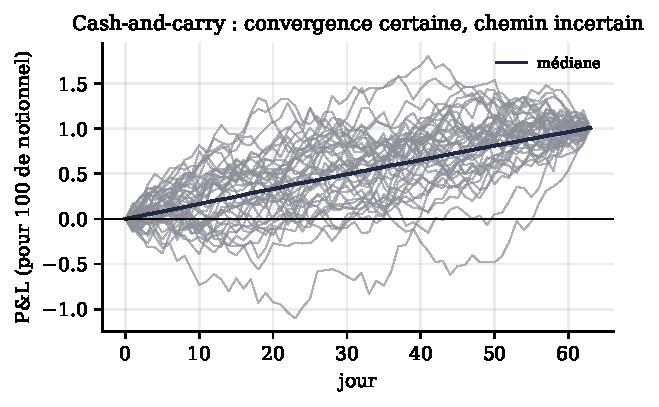
\includegraphics[width=0.62\textwidth]{ch14/cash_and_carry.pdf}
\caption{P\&L de 40 trajectoires d'un \emph{cash-and-carry} : toutes finissent au même gain, après des chemins différents.}
\label{c14:fig:cc}
\end{figure}

\paragraph{Lecture.} Le gain final est connu, mais si le comptant monte de 25\,\%, la jambe courte du future réclame 25 de marge \emph{en espèces}, alors que le gain de la jambe comptant est latent (sauf si l'on peut l'emprunter). Le risque d'un \emph{cash-and-carry} n'est pas le résultat final, c'est la liquidité nécessaire pour tenir jusqu'au bout. C'est exactement le mécanisme des limites de l'arbitrage de \citet{shleifer1997}.

% =====================================================================
\section{Les contrats perpétuels}
% =====================================================================

\subsection{Le mécanisme de \emph{funding}}

Un contrat perpétuel est un contrat à terme sans échéance, très répandu sur les plateformes de cryptomonnaies. Rien ne force sa convergence vers le comptant ; à la place, un paiement périodique (le \emph{funding}, souvent toutes les 8 heures, parfois toutes les heures) circule entre acheteurs et vendeurs. Quand le perpétuel cote au-dessus de l'indice comptant, le taux est positif et les positions longues paient les courtes ; quand il cote en dessous, l'inverse. Le taux combine en général une composante de prime (écart entre le perpétuel et l'indice) et une composante d'intérêt, avec des bornes ; \emph{la formule exacte dépend de chaque plateforme} et doit être lue dans sa documentation.

\citet{he2022perp} dérivent les prix d'absence d'arbitrage des perpétuels sans frictions et des bornes avec coûts de transaction ; ils trouvent que les écarts aux prix théoriques sont plus importants en crypto que sur les marchés de change traditionnels, qu'ils évoluent ensemble d'une cryptomonnaie à l'autre et qu'ils se réduisent avec le temps, et qu'une stratégie d'arbitrage fondée sur ces écarts aurait obtenu des ratios de Sharpe élevés.

\subsection{Le portage du \emph{funding}}

La stratégie la plus simple : acheter le comptant et vendre le perpétuel en même quantité. La position est neutre au prix ; elle encaisse le \emph{funding} tant qu'il est positif. Les risques :
\begin{enumerate}
\item le \emph{funding} peut devenir négatif pendant des périodes prolongées ;
\item la jambe courte est sur marge : une forte hausse peut la liquider, laissant la jambe comptant seule, non couverte ;
\item risque de contrepartie de la plateforme qui détient les deux jambes ou l'une d'elles ;
\item écart entre le perpétuel et le comptant au moment d'entrer et de sortir.
\end{enumerate}

\paragraph{Distance de liquidation.} Avec un levier $L$ sur la jambe courte (marge initiale $1/L$ du notionnel) et une marge de maintien $m$, la position est liquidée si le prix monte d'environ $1/L - m$ sans que la marge soit réapprovisionnée.

\begin{codebox}[ — E2, portage du \emph{funding} selon le levier]
\textbf{Protocole :} 5\,000 années simulées ; volatilité 60\,\% par an plus des sauts (environ quatre par an, d'écart-type 8\,\%) ; \emph{funding} quotidien autoregressif de moyenne $\approx10\,\%$ par an, négatif un jour sur trois ; marge réapprovisionnée chaque jour ; capital engagé = comptant + marge. \textbf{Résultats :}
\begin{center}\small
\begin{tabular}{rcccc}
\toprule
Levier & hausse liquidante (1 jour) & probabilité de liquidation & rendement moyen & quantile 5\,\% \\
\midrule
1 & 99,5\,\% & 0 & 5,0\,\% & $-2{,}4\,\%$\\
2 & 49,5\,\% & 0 & 6,6\,\% & $-3{,}2\,\%$\\
3 & 32,8\,\% & 0,2\,\% & 7,5\,\% & $-3{,}6\,\%$\\
5 & 19,5\,\% & 7,4\,\% & 7,9\,\% & $-4{,}0\,\%$\\
10 & 9,5\,\% & 71,7\,\% & 4,5\,\% & $-3{,}9\,\%$\\
\bottomrule
\end{tabular}
\end{center}
\end{codebox}

\paragraph{Lecture.} Le levier améliore le rendement sur capital tant qu'il n'expose pas à la liquidation ; au-delà, le rendement s'effondre, et le modèle sous-estime encore le danger : il suppose que la marge est réapprovisionnée chaque jour et ignore les mouvements intrajournaliers, l'écart entre perpétuel et comptant au moment de la liquidation, et la possibilité que la plateforme elle-même suspende les retraits.

% =====================================================================
\section{Étude de cas : les stratégies d'\texttt{atjte}}
% =====================================================================

\subsection{Le principe}

Le moteur \texttt{atjte} \citep{atjte} (chapitre~0, section~\ref{c0:atjte}) trade un écart entre deux instruments qui portent le même sous-jacent, par exemple un perpétuel ou un jeton adossé à l'or sur une plateforme crypto et le CFD XAUUSD chez un courtier MetaTrader~5 :
\[
s_t = P^{\text{plateforme}}_t - k\,P^{\text{MT5}}_t,
\]
où $k$ convertit les unités. Les ordres sont des ordres limites \emph{maker} sur la plateforme crypto, placés à $k\,P^{\text{MT5}}_{\text{bid}} + \text{niveau}$ à l'achat (et symétriquement à la vente), si bien qu'une exécution correspond à un écart égal au niveau visé, net de la fourchette du CFD. Chaque exécution est immédiatement couverte par un ordre au marché opposé sur MT5.

\subsection{Les stratégies fournies}

\begin{itemize}
\item \textbf{Niveaux fixes} : un ordre d'achat et un ordre de vente à des niveaux d'écart fixés.
\item \textbf{Grille} : plusieurs niveaux, pour accumuler une position quand l'écart s'éloigne.
\item \textbf{Bandes de Bollinger} : niveaux placés à la moyenne glissante de l'écart $\pm$ un multiple de son écart-type (fenêtre en minutes, échantillons à la seconde).
\item \textbf{Grille sur future daté} : le centre de la grille est la base \og juste\fg{} $=$ centre $+$ prix de référence $\times$ taux de portage annuel $\times$ jours restants$/365$, recalculée une fois par jour ; plus de nouvelle entrée à l'approche de l'échéance.
\end{itemize}

\subsection{Pourquoi le centre compte}

Quand la base a une composante déterministe (portage qui fond, écart de frais comme pour GLD/GLDM au chapitre~3, ou \emph{funding} moyen), où placer le centre des niveaux ?

\begin{codebox}[ — E3, centre fixe, moyenne glissante ou base théorique]
\textbf{Protocole :} base d'un future daté à un an avec portage de 4\,\% qui fond jusqu'à l'échéance, plus un écart AR(1) de demi-vie 3 jours autour de la base théorique ; trading sur 3 ans avec roulement annuel ; seuils $\pm1{,}5$ écart-type ; 4 pb par changement de position ; le P\&L inclut le portage (intérêts reçus ou payés), qui compense exactement la fonte de la base théorique. 300 simulations. \textbf{Résultats} (gain en pb par an) : centre fixe estimé sur un an $11{,}3$ (écart-type $14{,}4$) ; bandes de Bollinger sur 20 jours $73{,}3$ ($26{,}3$) ; base théorique $217{,}0$ ($34{,}1$).
\end{codebox}

\paragraph{Lecture.} Un centre fixe confond la fonte mécanique de la base avec un écart à corriger ; une moyenne glissante la suit mais avec retard, et son écart-type glissant est bruité ; un centre théorique isole exactement la partie aléatoire de l'écart. Quand une ancre théorique existe, il faut s'en servir : c'est ce que fait la stratégie de grille sur future daté d'\texttt{atjte}.

\begin{pitfall}
Sur la jambe CFD, le courtier facture des frais de financement de nuit (\emph{swap}) qui dépendent du sens de la position et de ses propres conditions ; sur un perpétuel, c'est le \emph{funding}. Ces deux portages ne se compensent pas forcément, et leur différence est un coût (ou un gain) permanent de la stratégie qu'il faut modéliser. Enfin, les règles des \emph{prop firms} interdisent ce type de couverture entre comptes ou plateformes : ces stratégies se déploient sur capital propre, chez des courtiers qui les acceptent.
\end{pitfall}

% =====================================================================
\section{Ce que la théorie apporte, et ses limites}
% =====================================================================

\paragraph{Apports.} Une ancre de prix exacte pour les contrats datés, une bande de non-arbitrage avec frictions, une compréhension du \emph{funding} comme substitut de la convergence, et un critère de levier fondé sur la distance de liquidation.

\paragraph{Limites.} Les perpétuels n'ont pas d'ancre stricte : l'écart peut rester large longtemps. Le risque de contrepartie des plateformes est réel et non diversifiable à l'intérieur d'une même plateforme. Les règles de marge, de liquidation et de \emph{funding} changent d'une plateforme à l'autre et dans le temps. Les besoins de liquidité peuvent forcer une sortie avant la convergence.

% =====================================================================
\section{Fiche à recopier au tableau blanc}
% =====================================================================

\begin{whiteboard}
\begin{itemize}[leftmargin=1.2em]
\item \textbf{Portage :} $F = Se^{(r-q)T}$ ; base $F - S\to0$ à l'échéance.
\item \textbf{Bande :} $Se^{(r_l-q)T} - c' \le F \le Se^{(r_b-q)T} + c$.
\item \textbf{Cash-and-carry :} long comptant financé, court future ; gain final fixé, besoin de marge variable.
\item \textbf{Funding :} longs paient les courts si perpétuel $>$ indice ; formule propre à chaque plateforme.
\item \textbf{Liquidation :} hausse de $\approx 1/L - m$ sur la jambe courte.
\item \textbf{atjte :} $s_t = P^{\text{plat}} - kP^{\text{MT5}}$ ; maker sur la plateforme, taker sur MT5 ; centre théorique $=$ référence $\times$ portage $\times$ jours$/365$.
\end{itemize}
\end{whiteboard}

% =====================================================================
\section{Exercices}
% =====================================================================

\begin{exercise}
L'or comptant vaut 4\,000, le taux est de 4\,\%, le coût de stockage de 0,1\,\% par an. Quel est le prix théorique du contrat à 6 mois ? Quelle est la base en dollars et en points de base ?
\end{exercise}

\begin{exercise}
Le \emph{funding} moyen est de 0,01\,\% toutes les 8 heures. Calculez le rendement annuel brut d'un portage sans levier, puis le rendement sur capital avec un levier de 3 sur la jambe courte.
\end{exercise}

\begin{exercise}
Justifiez la formule de distance de liquidation $1/L - m$ à partir de la définition de la marge.
\end{exercise}

\begin{exercise}[à coder]
Dans E2, remplacez le réapprovisionnement quotidien de la marge par un réapprovisionnement hebdomadaire. Comment change la probabilité de liquidation pour un levier de 3 ?
\end{exercise}

\begin{exercise}[à coder]
Reprenez E3 en ajoutant un écart constant de 10 pb par an entre le \emph{swap} du CFD et le portage de la plateforme. Comment faut-il modifier le centre théorique ?
\end{exercise}

% =====================================================================
\section{Pour aller plus loin}
% =====================================================================

\begin{toread}
\begin{itemize}[leftmargin=1.2em]
\item \citet{hull2022} : les chapitres sur la détermination des prix à terme et sur les futures de matières premières.
\item \citet{he2022perp} : théorie des prix des perpétuels et mesure des écarts.
\item \citet{shleifer1997} : pourquoi un arbitrage à gain final certain peut tout de même échouer.
\item Le code d'\texttt{atjte} \citep{atjte} : \texttt{strategy\_types/arb/bollinger\_bot} et \texttt{grid\_futures\_bot}, et le module \texttt{engines/common/ratio.py} pour le contrôle du ratio $k$.
\end{itemize}
\end{toread}

\section{Scripts du chapitre}
\noindent\texttt{code/ch14/ch14\_basis\_funding.py} : E1 (figure~\ref{c14:fig:cc}), E2, E3.
